%Dokumententyp
\documentclass[a4paper]{article}

\usepackage[a4paper,left=2cm, right=3cm, top=2cm]{geometry}

%Kodierung
\usepackage[utf8]{inputenc}
\usepackage[T1]{fontenc}

%Grafiken einbinden
\usepackage{graphicx}
\usepackage{subfigure} 

%Position von Grafiken und Tabellen erzwingen:
\usepackage{float}

%URLs im Literaturverzeichnis
\usepackage{url}

\usepackage{amsmath}

%Vektoren einfacher angeben:
\newcommand{\vektor}[1]{\left( \begin{array}{c} #1 \end{array} \right) }


%Schriftart Arial:
% \usepackage{helvet}

%Figures with text around it:
\usepackage{wrapfig}

\usepackage{listings}

%seitennummern rechts:
% \usepackage{fancyhdr}
% \fancyhf{} % clear all header and footers
% \renewcommand{\headrulewidth}{0pt} % remove the header rule
% \rfoot{\thepage}
% \fancypagestyle{plain}{%redefining plain pagestyle
% \fancyhf %clear all headers and footers fields
% \fancyhead[R]{\thepage} %prints the page number on the right side of the header
% }

%Schriftart Times New Roman "like"
\usepackage{txfonts}

%Sprache
\usepackage[german]{babel}

%Checkmarks: (usage: \checkmark)
\usepackage{dingbat}

\usepackage{listings}
\usepackage{color}
\definecolor{javared}{rgb}{0.6,0,0} % for strings
\definecolor{javagreen}{rgb}{0.25,0.5,0.35} % comments
\definecolor{javapurple}{rgb}{0.5,0,0.35} % keywords
\definecolor{javadocblue}{rgb}{0.25,0.35,0.75} % javadoc
 
\lstset{language=Java,
basicstyle=\ttfamily,
keywordstyle=\color{javapurple}\bfseries,
stringstyle=\color{javared},
commentstyle=\color{javagreen},
morecomment=[s][\color{javadocblue}]{/**}{*/},
numbers=left,
numberstyle=\tiny\color{black},
stepnumber=1,
numbersep=5pt,
tabsize=4,
showspaces=false,
lineskip={-1.5pt},
showstringspaces=false}

%Tabellenextras
\usepackage{tabularx}

%Zeilenabstand 1.5
\linespread{1.5}
\usepackage{setspace}

%URLs
\usepackage{url}

%
\usepackage{cancel}

%Figure Captions mit Fußnoten
\usepackage{footnote}
%\setlength{\parindent}{0pt} 

%Graphen/Trees zeichnen:
\usepackage{tikz}
\newcommand*\circled[1]{\tikz[baseline=(char.base)]{
            \node[shape=circle,draw,inner sep=2pt] (char) {#1};}}


%itemize items richtig ausrichten (nicht links überlappen!)
% \setlist{leftmargin=0}

% %%%%TITELSEITE%%%%%%(
% \title{ Konzept und Implementierung\\ eines Systems zur \\Anforderung und Verwaltung von virtuellen privaten Clustern}
% \author{\textbf{\large Bachelorarbeit}}
% 
% \date{zur Erlangung des akademischen Grades Bachelor of Science an der Universität Paderborn im Fachbereich Informatik im Studiengang Bachelor Informatik}

% %%%%TITELSEITE%%%%%%)

% \pagestyle{fancy}
\begin{document}

\title{Algorithmische Geometrie - Sommersemester 2015\\
       10. Aufgabenblatt }
\author{Simon Koennecke und Felix Bröker}
\date{}
\maketitle

\section*{Aufgabe 1}
Gegeben sei eine Punktmenge $P = \{ (x,y) | x,y \in \mathcal{R} \} \subset \mathcal{R}^2$.
Es ist die maximale Anzahl von Punkten $p \in P$ gesucht, die auf einer gemeinsamen Geraden $g$ liegen.

Zur Lösung der Aufgabe formulieren wir die Problemstellung in eine duale Darstellung wie folgt um:
Gegeben sei eine Menge von Geraden $G = \{a*x -y = b | a,b \in \mathcal{R} \wedge (x,y) \in P \}$.
Es ist die maximale Anzahl von Geraden $g \in G$ gesucht, die sich in einem gemeinsamen Punkt $q$ schneiden.
Sind dieser Punkt $q = (q_a, q_b)$ und die in diesem Punkt schneidenden Geraden $g \in G$ ermittelt, lassen sich über
die Dualitätsabbildung:

\begin{align}
q = (q_a, a_b) &\longmapsto l: y = q_a * x - q_b\\
g:  a*x -y = b &\longmapsto p = (x,y)
\end{align}

die ursprünglich gesuchte Gerade und Punkte direkt ermitteln. 

Unser folgender Algorithmus arbeitet also auf der dualen Darstellung und bestimmt Punkt $q$:
\vspace*{1cm}

 Initialisiere einen AVL-Baum $H$ und Variable $MAX = 0$.
 (Jeder Knoten des Baums $H$ soll dabei sowohl einen Schnittpunkt $s$ 
 als auch einen Zähler $c$ speichern können)
 
 Für alle $g \in G$:
 \begin{itemize}
  \item Durchlaufe alle $g' \in G \setminus \{g\}$ 
  \begin{itemize}
   \item Betrachte die Geraden $g$ und $g'$
   \begin{itemize}
       \item Fall 1 ($g$ und $g'$ liegen aufeinander):
	Dieser Fall ist aufgrund der Konstruktion von $G$ nicht möglich.
       \item Fall 2 ($g$ und $g'$ liegen parallel zueinander):
	Fahre mit nächster Schleifeniteration fort.
       \item Fall 3 ($g$ und $g'$ haben einen Schnittpunkt $s$):
       
	Aktualisiere $H$ folgendermaßen:
	\begin{itemize}
	 \item Fall 1 ($s \in H$):
	 Erhöhe den Zähler $c$ von $s$ in $H$ um 1.
	 Sollte $c$ jetzt $> MAX$ sein, aktualisiere $MAX$ mit $MAX = c$.
	 \item Fall 2 ($s \notin H$):
	 Füge $s$ mit dem Zählerwert $c = 1$ zu $H$ hinzu.
	 Sollte $c$ jetzt $> MAX$ sein, aktualisiere $MAX$ mit $MAX = c$.
	\end{itemize}

   \end{itemize}
 
  \end{itemize}
 \end{itemize}
 Gebe Wert der Variablen $MAX$ aus.
 
 \subsection*{Laufzeit}
 Die Laufzeit lässt sich wie folgt abschätzen:
 
 \begin{itemize}
  \item Das Durchlaufen aller Geraden benötigt $\mathcal{O}(n)$ Zeit
    \item Das jeweilige Vergleichen mit allen anderen Geraden benötigt ebenfalls $\mathcal{O}(n)$ Zeit.
  \item Die Bestimmung des Falles bei Betrachtung der Geraden $g$ und $g'$ geht in $\mathcal{O}(1)$ Zeit.
  \item Die Fälle 1 und 2 können dabei ebenfalls in $\mathcal{O}(1)$ Zeit bearbeitet werden.
  \item Der 3. Fall benötigt $\mathcal{O}(\log n)$ Zeit. 
  
  Denn das Einfügen in den AVL-Baum ist bekanntermaßen in $\mathcal{O}(\log n)$ Zeit möglich.
  Das Aktualisieren des Zählers $c$ eines Schnittpunkts $s$ kann durch das Suchen von $s$ in $H$
  und anschließendes Inkrementieren des Zählers $c$ in $\mathcal{O}(\log n)$ durchgeführt werden.
  
 \end{itemize}
 
 Daraus resultiert eine Gesamtlaufzeit von $\mathcal{O}(n) * (\mathcal{O}(n) * (\underbrace{\mathcal{O}(1) + \mathcal{O}(\log n)}_{\mathcal{O}(\log n)})) = \mathcal{O}(n^2 \log n)$



\section*{Aufgabe 2}

Zur Bearbeitung der Aufgabe greifen wir auf das "`Upper bound theorem"' (McMullen, Shephard 1971) zurück.
Dieses sagt aus, dass zyklische Polytope unter allen konvexen Polytopen genau diejenigen sind, welche eine größtmögliche Anzahl von Facetten (in Bezug auf eine Dimension $d$ und eine Anzahl von
Ecken $n$) besitzen.

Ein $d$-dimensionales zyklisches Poplytop ist über die so genannte Momentenkurve im $\mathcal{R}^d$ definiert. Die Momentenkurve ist definiert als:

$$x: \mathcal{R} \rightarrow \mathcal{R}^d, x(t) := [t, t^2, \dots, t^d]^T$$

und das $d$-dimensionale zyklische Polytop (Dimension $d$ mit $n$ Ecken) dann als:

$$C(n,d) := conv\{x(t_1), x(t_2), \dots, x(t_n) \quad|\quad n > d \geq 2, t_1 < t_2 < \dots < t_n\}$$

Entsprechend der Aufgabenstellung wählen wir für ein beliebiges $n \in \mathcal{N}$ nun
einfach $n$ disjunkte Punkte auf der 4-dimensionalen Momentenkurve. 
Die darüber definierte konvexe Hülle ist folglich genau jenes zyklisches Polytop $C(n,4)$, 
für welches wir wissen, dass es die maximale Anzahl von Facetten unter allen konvexen Polytopen
mit $n$ Ecken in 4 Dimensionen aufweist. 

Da jedes zyklische Polytop $C(n,d)$ $k$-nachbarschaftlich mit $k = \lfloor\frac{d}{2}\rfloor $ ist, also im $4
d$-Fall
$2$-nachbarschaftlich, wissen wir, dass alle 2er-Kombinationen von Ecken des Polytops
(also alle Ecken mit jeweils allen anderen Ecken) über eine Kante verbunden sind. Die Anzahl der Kanten, sprich der d-3 dimensionalen
Facetten, lässt sich demnach über den Binomialkoeffizienten mit $\binom{n}{2} = \frac{n!}{2! * (n-2)!}
= \frac{n * (n-1)}{2} = \frac{n^2 - n}{2} = \mathcal{O}(n^2)$ abschätzen. 

\section*{Aufgabe 3}
\subsection*{(a)}

Da wir innerhalb der Vorlesung keinen inkrementellen Algorithmus zur Konstruktion der konvexen Hülle im $\mathcal{R}^3$ kennengelernt bzw. analysiert haben,
stellen wir im Folgenden zunächst einen selbst entwickelten Algorithmus vor. Dieser Algorithmus erfüllt die geforderte Laufzeit $\Omega(n^2)$ für beliebige
Eingaben und Einfügereihenfolgen. Da aber die Aufgabenstellung impliziert, dass der gegebene Algorithmus eine (zumindest erwartete) Laufzeit besser als $\Omega(n^2)$
besitzt, haben wir recherchiert und einen entsprechenden randomisierten inkrementellen Algorithmus zur Berechnung der konvexen Hülle im $\mathcal{R}^3$ mit 
erwarteter Laufzeit von $\mathcal{O}(n \log n)$ gefunden (Quelle: Mark de Berg et al. - "`Computational Geometry"', 2008, Springer-Verlag).
Dieser wird auch anschaulich unter folgender URL animiert und beschrieben: \url{http://www.eecs.tufts.edu/~mhorn01/comp163/}. 
Wir betrachten für die Bearbeitung der Aufgabe jedoch die nicht randomisierte Version dieses Algorithmus, d.h. die definierte Einfügereihenfolge
wird beachtet.

\subsection*{Inkrementeller Algorithmus mit Laufzeit $\Omega(n^2)$ unabhängig von der Eingabe und Einfügereihenfolge}
Sei die Punktmenge $S \subset \mathcal{R}^3$ gegeben, $|S| = n$ und $F$ die Facetten der konvexen Hülle. Der Schnitt der negativen Halbräume der Facetten aus $F$ beschreiben das Innere der konvexen Hülle. 
Zur Vereinfachung nehmen wir an, dass die Punkte aus $S$ in allgemeiner Lage sind. Somit spannen die ersten vier Punkte ein Tetraeder und die vier Facetten des Tetraeders werden in $F$ gespeichert. Anschließend werden die Punkte inkrementell hinzugefügt unter Anwendung des folgenden Algorithmus: 

\begin{itemize}
	\item Solange $S \neq \varnothing$
	\begin{itemize}	
		\item Wähle einen Punkt $p \in S$ und aktualisiere $S$ mit $S = S \setminus \{p\}$
		\item Fall 1: $p$ liegt in der konvexen Hülle von $F$, weiter mit dem ersten Schritt.
		\item Fall 2: $p$ liegt außerhalb der konvexen Hülle von $F$.
	\begin{itemize}
		\item Entferne die Facetten aus $F$ bei denen $p$ im positiven Halbraum liegt.
		\item Durchlaufe wiederholt die Facetten aus $F$ und wähle von den Facetten alle Kanten $ e = (i,j) $, welche keine Nachbarfacette haben.
		Füge jeweils die neue Facette mit den Eckpunkten $i,j$ und $p$ zu $F$ hinzu, wobei die Nachbarschaftsbeziehungen entsprechend aktualisiert werden. 
	\end{itemize}
	\end{itemize}
\end{itemize}


\subsubsection*{Laufzeit}

Die Prüfung, ob ein Punkt $p$ in der konvexen Hülle $F$ liegt, kann wie folgt realisiert werden: Der Punkt $p$ liegt im negativen Halbraum aller Facetten aus $F$. Dies kann in $\mathcal{O}(n)$ Zeit geprüft werden, da die Anzahl der Facetten zu den Punkten durch die Eulerformel in linearer Abhängigkeit stehen. Das Entfernen der Facetten, bei dem der Punkt $p$ im positiven Halbraum liegt, benötigt $\mathcal{O}(n)$ Zeit. Das finden der Eckpunkte von Kanten ohne Nachbarn wird durch wiederholtes Durchlaufen aller übrig geblieben Facetten ermöglicht und benötigt ebenfalls $\mathcal{O}(n)$ Zeit. Insgesamt wird $\mathcal{O}(3n)$ Zeit benötigt. Dies Vorgehen wird für $n$ Punkte wiederholt und daraus resultiert die Gesamtlaufzeit $\Omega(n^2)$.

\subsubsection*{Speicherplatzbedarf}

Im Initialzustand sind die Facetten $F$ Dreiecke und beim inkrementellen Hinzufügen der Punkte werden nur Dreiecke als Facetten aufgenommen. Da die Punkte in allgemeiner Lage sind können die Facetten nur Dreiecke sein. Daher hat jede Facette 3 Ecken und wir wissen, dass jeder Punkt aus der Menge $S$ linear viele Facetten nach der Eulerformel (Dualität planarer Graph) hat. Daraus resultiert der Speicherplatzbedarf von $\mathcal{O}(n)$.

\subsection*{Alternativer Algorithmus mit erwarteter Laufzeit von $\mathcal{O}(n \log n)$}
In der von de Berg et al. beschriebenen Laufzeitanalyse wird die erwartete Anzahl der in einem Schritt $i$ neu hinzuzufügenden Facetten nach oben mit einer Konstante ($c = 6$) abgeschätzt.
Dies folgt aus einer Betrachtung des mittleren Knotengrades im Schritt $i$. 

Wie wir nun zeigen, können wir über die folgend definierte Eingabe und Einfügereihenfolge diesen Wert auf einen von $n$ linear abhängigen Wert erhöhen/"`verschlimmern"'.

Dazu konstruieren wir eine Eingabe der Größe $n$, wobei wir $\lfloor\frac{n}{2}\rfloor$ Punkte auf einem Kreisrand in der $x-y-Ebene$ anordnen. 
Sei $m = (x_m,y_m)$ der Mittelpunkt dieses Kreises. Die verbliebenen $\lceil\frac{n}{2}\rceil$ Punkte sind beschrieben durch $(x_m, y_m, z_i)$. Es gilt dabei dass $z_i < z_{i+1}$.
Das heißt wir ordnen die Hälfte der Punkte auf einem Kreis in der Ebene an und wählen danach immer Punkte über dem Kreismittelpunkt, welche bezgl. $z$ immer weiter 
"`in die Höhe wachsen"'. Die Einfügereihenfolge kann in der beschriebenen Weise übernommen werden.

Dann ergibt sich folgende Änderung für die erwartete Laufzeit eines Schrittes $i$:

Das Erstellen des Initialzustands, d.h. die Konstruktion des Tetraeders benötigt $\mathcal{O}(n)$ Zeit.
Das Einfügen der $\mathcal{O}(\frac{n}{2})$ ersten Punkte (die auf dem Kreis liegen) benötigt jeweils konstante Zeit,
da pro Punkt jeweils nur konstant viele neue Facetten erstellt/gelöscht werden. also insgesamt auch $\mathcal{O}(\frac{n}{2})$ Zeit.
Für die verbleibende Punktmenge benötigen wir $\mathcal{O}((\frac{n}{2})^2)$ Zeit. Denn aufgrund der Lage der ersten $\mathcal{O}(\frac{n}{2})$ Punkte
müssen wir für jeden neu hinzugefügten Punkt  $\mathcal{O}(\frac{n}{2})$ neue Flächen hinzufügen bzw. löschen. 

Insgesamt haben wir eine Laufzeit von  $\mathcal{O}(n) + \mathcal{O}(\frac{n}{2}) + \mathcal{O}((\frac{n}{2})^2) = \mathcal{O}(\frac{n^2}{4}) = \Omega(n^2) $.


\subsection*{(b)}
Zur Bearbeitung der Aufgabe betrachten wir den Algorithmus aus der Vorlesung und lassen dabei jedoch die Randomisierung außer Acht.
Die Eingabemenge wählen wir mit $\frac{n}{2}$ parallelen, gleichlangen Strecken. Die anderen $\frac{n}{2}$ Strecken sind ebenfalls parallel und gleich lang, liegen jedoch
orthogonal so zu den ersten $\frac{n}{2}$  Strecken, dass sich eine jede Strecke mit jeweils $\frac{n}{2}$ Strecken schneidet.

\begin{figure}[!htb]
\subfigure[Illustration der gewählten Eingabestrecken]{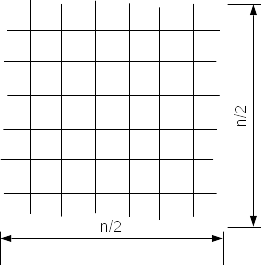
\includegraphics[width=0.25\textwidth]{aufgabe3b}} 
\end{figure} 


\textbf{Satz aus der Vorlesung:}

\textbf{Die Trapezierung einer Menge von $n$ Strecken mit obigem randomisierten inkrementellen Algorithmus hat die erwartete Laufzeit
$\mathcal{O}(n\log n + k)$, wobei $k$ die Anzahl der Schnittpunkte ist.}


Beim Einfügen der ersten $\frac{n}{2}$ vertikalen Strecken beträgt die Anzahl der Schnittpunkte jeweils 0 . Beim Einfügen der horizontalen Strecken jeweils $\frac{n}{2}$.
Damit haben wir insgesamt genau $\frac{n}{2} * \frac{n}{2} = \mathcal{O}(\frac{n^2}{4}) = \mathcal{O}(n^2)$ Schnittpunkte.

Die Laufzeit beträgt somit $\mathcal{O}(n \log n + n^2) = \Omega(n^2)$.
  

\end{document}

